% Options for packages loaded elsewhere
\PassOptionsToPackage{unicode}{hyperref}
\PassOptionsToPackage{hyphens}{url}
\PassOptionsToPackage{dvipsnames,svgnames*,x11names*}{xcolor}
%
\documentclass[
  11pt,
]{article}
\usepackage{lmodern}
\usepackage{setspace}
\usepackage{amsmath}
\usepackage{ifxetex,ifluatex}
\ifnum 0\ifxetex 1\fi\ifluatex 1\fi=0 % if pdftex
  \usepackage[T1]{fontenc}
  \usepackage[utf8]{inputenc}
  \usepackage{textcomp} % provide euro and other symbols
  \usepackage{amssymb}
\else % if luatex or xetex
  \usepackage{unicode-math}
  \defaultfontfeatures{Scale=MatchLowercase}
  \defaultfontfeatures[\rmfamily]{Ligatures=TeX,Scale=1}
\fi
% Use upquote if available, for straight quotes in verbatim environments
\IfFileExists{upquote.sty}{\usepackage{upquote}}{}
\IfFileExists{microtype.sty}{% use microtype if available
  \usepackage[]{microtype}
  \UseMicrotypeSet[protrusion]{basicmath} % disable protrusion for tt fonts
}{}
\makeatletter
\@ifundefined{KOMAClassName}{% if non-KOMA class
  \IfFileExists{parskip.sty}{%
    \usepackage{parskip}
  }{% else
    \setlength{\parindent}{0pt}
    \setlength{\parskip}{6pt plus 2pt minus 1pt}}
}{% if KOMA class
  \KOMAoptions{parskip=half}}
\makeatother
\usepackage{xcolor}
\IfFileExists{xurl.sty}{\usepackage{xurl}}{} % add URL line breaks if available
\IfFileExists{bookmark.sty}{\usepackage{bookmark}}{\usepackage{hyperref}}
\hypersetup{
  pdftitle={Semiparametric estimation for time series: a frequency domain approach based on optimal transportation theory},
  colorlinks=true,
  linkcolor=Maroon,
  filecolor=Maroon,
  citecolor=Blue,
  urlcolor=blue,
  pdfcreator={LaTeX via pandoc}}
\urlstyle{same} % disable monospaced font for URLs
\usepackage[margin=1in]{geometry}
\usepackage{graphicx}
\makeatletter
\def\maxwidth{\ifdim\Gin@nat@width>\linewidth\linewidth\else\Gin@nat@width\fi}
\def\maxheight{\ifdim\Gin@nat@height>\textheight\textheight\else\Gin@nat@height\fi}
\makeatother
% Scale images if necessary, so that they will not overflow the page
% margins by default, and it is still possible to overwrite the defaults
% using explicit options in \includegraphics[width, height, ...]{}
\setkeys{Gin}{width=\maxwidth,height=\maxheight,keepaspectratio}
% Set default figure placement to htbp
\makeatletter
\def\fps@figure{htbp}
\makeatother
\setlength{\emergencystretch}{3em} % prevent overfull lines
\providecommand{\tightlist}{%
  \setlength{\itemsep}{0pt}\setlength{\parskip}{0pt}}
\setcounter{secnumdepth}{5}
\usepackage{caption}
\captionsetup[figure]{font=footnotesize,margin=9pt,labelfont=bf,textfont=it}
\captionsetup[table]{font=footnotesize,margin=9pt,labelfont=bf,textfont=it}
\ifluatex
  \usepackage{selnolig}  % disable illegal ligatures
\fi
\newlength{\cslhangindent}
\setlength{\cslhangindent}{1.5em}
\newlength{\csllabelwidth}
\setlength{\csllabelwidth}{3em}
\newenvironment{CSLReferences}[2] % #1 hanging-ident, #2 entry spacing
 {% don't indent paragraphs
  \setlength{\parindent}{0pt}
  % turn on hanging indent if param 1 is 1
  \ifodd #1 \everypar{\setlength{\hangindent}{\cslhangindent}}\ignorespaces\fi
  % set entry spacing
  \ifnum #2 > 0
  \setlength{\parskip}{#2\baselineskip}
  \fi
 }%
 {}
\usepackage{calc}
\newcommand{\CSLBlock}[1]{#1\hfill\break}
\newcommand{\CSLLeftMargin}[1]{\parbox[t]{\csllabelwidth}{#1}}
\newcommand{\CSLRightInline}[1]{\parbox[t]{\linewidth - \csllabelwidth}{#1}\break}
\newcommand{\CSLIndent}[1]{\hspace{\cslhangindent}#1}

\title{Semiparametric estimation for time series: a frequency domain
approach based on optimal transportation theory}
\author{Manon Felix\\
Advisor: Prof.~Davide La Vecchia}
\date{May 2021}

\begin{document}
\maketitle
\begin{abstract}
In this master thesis, we make use of some results available in the
optimal transportation literature to develop a novel methodology for
parameters estimation in time series models based. The key idea is to
use the Wasserstein distance and Sinkhorn divergence to derive minimum
distance (or divergence) estimators for short- and long-memory time
series models. Working on the Fourier transform of a time series we
conduct inference in the frequency domain: we compute the
distance/divergence between the empirical distribution of the
standardized periodogram ordinates and their theoretical distribution,
as implied by standard asymptotic theory. To study the properties of
these new estimators, we perform several Monte-Carlo simulations. Our
numerical results suggest that the estimators belonging to our novel
class are root-\(n\) consistent. Their performance, in terms of Mean
Squared-Error, is similar to the one yielded by the state-ofthe-art
estimation method (Whittle's estimator) in the case of short- and
long-memory Gaussian process. Furthermore, when the underlying
innovation density of a long-memory process is skewed, our estimators
overperform the Whittle's estimator.
\end{abstract}

\setstretch{1.5}
\newpage

\tableofcontents

\newpage

\hypertarget{introduction}{%
\section{Introduction}\label{introduction}}

\hypertarget{motivation}{%
\subsection{Motivation}\label{motivation}}

The aim of this master thesis is to combine some results from optimal
transport theory with the statistical analysis time series analysis.
Working with the frequency domain approach, we aim at developing a novel
methodology for estimating the parameters of a univariate stochastic
process.

We do not rely on the standard information divergence-based methods,
among which the standard maximum likelihood estimator approach, and
consider instead the mathematical theory of optimal measure
transportation.

The optimal transport theory has been applied in many research areas,
like e.g.~mathematics, differential geometry, partial differential
equations and applied mathematics (see e.g.
\protect\hyperlink{ref-santambrogio2015optimal}{Santambrogio}
(\protect\hyperlink{ref-santambrogio2015optimal}{2015}) and
\protect\hyperlink{ref-villani2009optimal}{Villani}
(\protect\hyperlink{ref-villani2009optimal}{2009})). The Wasserstein
distance is also useful for contrasting complex objects and can be
applied to signal processes and engineering (see e.g.
\protect\hyperlink{ref-kolouri2017optimal}{Kolouri et al.}
(\protect\hyperlink{ref-kolouri2017optimal}{2017})). We refer to
\protect\hyperlink{ref-bernton2019parameter}{Bernton et al.}
(\protect\hyperlink{ref-bernton2019parameter}{2019}) for an survey of
the Wasserstein distance. Many data analysis techniques in computer
vision, imaging (e.g.~for color/texture processing or histograms
comparisons), and more general machine learning problems about
regression, classification, and generative modeling are often based on
optimal transportation theory (see
\protect\hyperlink{ref-peyre2019computational}{Peyré, Cuturi, and
others} (\protect\hyperlink{ref-peyre2019computational}{2019})). For an
overview on statistical use of the optimal transportation see
\protect\hyperlink{ref-panaretos2020invitation}{Panaretos and Zemel}
(\protect\hyperlink{ref-panaretos2020invitation}{2020}) and for a
book-length discussion see
\protect\hyperlink{ref-ambrosio2013user}{Ambrosio and Gigli}
(\protect\hyperlink{ref-ambrosio2013user}{2013}). Recently, the
Wasserstein distance has become popular specially for inference in
generative adversarial networks (see e.g.,
\protect\hyperlink{ref-arjovsky2017wasserstein}{Arjovsky, Chintala, and
Bottou} (\protect\hyperlink{ref-arjovsky2017wasserstein}{2017})).

However, to the best of our knowledge, only a limited number of papers
has been investigating the use of the optimal transport theory in the
statistical analysis of time series analysis (see
\protect\hyperlink{ref-ni2020conditional}{Ni et al.}
(\protect\hyperlink{ref-ni2020conditional}{2020})). Our purpose is to
fill this gap in the literature and study the applicability of the
Wasserstein distance (or, more generally, of some results from optimal
transportation theory) for the statistical analysis of time series, via
frequency domain techniques. The key argument for moving from the time
domain to the frequency domain is that we are dealing with data that are
independent and identically distributed (i.i.d). The assumption of
i.i.d. data facilitates, as it is often the case in statistics, the
estimation of parameters in a model.

We propose a novel class of minimum distance estimator (see
\protect\hyperlink{ref-basu2019statistical}{Basu, Shioya, and Park}
(\protect\hyperlink{ref-basu2019statistical}{2019})) by minimizing the
distance between the theoretical and empirical distribution of the
standardized periodogram ordinates (SPOs). This program is supported by
the fact that the method to replace the maximum likelihood estimator
with minimum Wasserstein distance has already been applied, for instance
in astronomy and climate science (see
\protect\hyperlink{ref-bernton2019parameter}{Bernton et al.}
(\protect\hyperlink{ref-bernton2019parameter}{2019})). Additionally,
consistency properties of estimators based on the Wasserstein distance
has already been studied by
\protect\hyperlink{ref-bassetti2006minimum}{Bassetti, Bodini, and
Regazzini} (\protect\hyperlink{ref-bassetti2006minimum}{2006}) and
\protect\hyperlink{ref-bernton2019parameter}{Bernton et al.}
(\protect\hyperlink{ref-bernton2019parameter}{2019}). In our case, we
study the properties (bias, variance, consistency, etc.) of our new
estimators by means of Monte-Carlo experiments and compare them to the
state-of-the-art estimator, the Whittle's estimator (see
\protect\hyperlink{ref-whittle1953estimation}{Whittle}
(\protect\hyperlink{ref-whittle1953estimation}{1953})). We analyze our
results for several types of distribution (standard, heavy-tailed and
skewed) and focus mainly on large sample sizes to satisfy the i.i.d
conditions. Our results are promising and open the possibility of
further research.

\hypertarget{organization}{%
\subsection{Organization}\label{organization}}

In the first chapter, we review the main concepts of the optimal
transport theory and provide the definitions and key mathematical tools
necessary to understand our methodological development. In the second
chapter, we briefly recall the Whittle's estimation theory and the key
related results. Then, we introduce our novel estimators and compare
them to the state-of-art estimator (Whittle). We conclude mentioning
some possible research's directions which can make use of this thesis as
a stepston. The R-codes needed to reproduce the exercises/plots/tables
included in this thesis are available on Github at the link
\url{https://github.com/ManonFelix/Semidiscrete_estimation_ts}.

\hypertarget{measure-transportation}{%
\section{Measure transportation}\label{measure-transportation}}

This chapter aims to explain the main principles behind the theory of
optimal transport. The original formulation of the optimal transport
problem was given by \protect\hyperlink{ref-monge1781memoire}{Monge}
(\protect\hyperlink{ref-monge1781memoire}{1781}). He proposed a way to
calculate the most effective strategy for moving a large amount of sand
from one place to another with the least amount of effort required. In
mathematical terms, given a source measure \(\mu\), target measure
\(\nu\) supported on sets \(X\) and \(Y\) respectively and a
transportation cost function \(c(x,y)\) the goal is to find a transport
map \(T:X \rightarrow Y\) such as

\[\min _{\nu=T_{\#} \mu} \int_{X} c(x, T(x)) \mathrm{d} \nu(x)\]

where the constraint
\(\mu(T^{-1}(A) = \nu(A) \implies \nu=T_{\#} \mu \ , \forall A\) ensures
that all the mass from \(\mu\) is transported to \(\nu\) by the map
\(T\).

The notation \(\nu=T_{\#} \mu\) means that the map \(T\) pushes forward
\(\mu\) to a new measure \(\nu\) and therefore \(T_{\#}\) is called the
pushforward operator.

Monges problem (defined using \(c(x, y)=|x-y|)\) remained open until the
\(1940 \mathrm{~s}\), when it was revisited by
\protect\hyperlink{ref-kantorovich1942translocation}{Kantorovich}
(\protect\hyperlink{ref-kantorovich1942translocation}{1942}). In his
reformulation, he seeks for a transport plan and allows mass splitting.
Therefore, he proposed to compute how much mass gets moved from \(x\) to
\(y\) and define a joint measure (a coupling)
\(\pi \in \mathcal{P}\left(\mathbb{R}^{d}, \mathbb{R}^{d}\right)\) which
satisfies for all \(A, B \in \mathcal{B}\left(\mathbb{R}^{d}\right)\):
\(\pi\left(A \times \mathbb{R}^{d}\right)=\mu(A), \ \pi\left(\mathbb{R}^{d} \times B\right)=\nu(B).\)
We denote by \(\Pi(\mu, \nu)\) the set of transport plans between
\(\mu\) and \(\nu\) (i.e.~couplings). Then, \(p\)-Wasserstein distance
is defined as

\begin{equation}
W_{p}(\mu, \nu)=\left(\min _{\pi \in \Pi(\mu, \nu)} \int_{\mathbb{R}^{d} \times \mathbb{R}^{d}}|x-y|^{p} d \pi(x, y)\right)^{\frac{1}{p}}.
\end{equation}

Obtaining a closed-form expression for \(W_{p}\) is typically
impossible. However, the case of one dimensional probability densities,
say \(f_{S}(x)\) and \(f_{T}(x)\) with cumulative distribution functions
\(F_{S}(x)\) and \(F_{T}(x)\), is specifically interesting as the
Wasserstein distance (a.k.a the Earth Mover's Distance (EMD)) has the
following expression

\begin{equation}
\mathcal{W}_{1}(\mu, \nu)=\int_{\mathbb{R}}\left|F_{S}(x)-F_{T}(x)\right| d x
\label{eq:wass_1}
\end{equation}

The possibility of using this closed-formed solution to conduct
inference on time series motivates the thesis.

\protect\hyperlink{ref-cuturi2013sinkhorn}{Cuturi}
(\protect\hyperlink{ref-cuturi2013sinkhorn}{2013}) introduced a modified
version of the Wasserstein distance:

\begin{equation}
W_{\lambda}(\mu, \nu) =\int_{x, y} C(x, y) \mathrm{d} \pi(x, y)+ \lambda \int \log \left(\frac{\pi(x, y)}{\mathrm{d} \mu(x) \mathrm{d} \nu(y)}\right) \mathrm{d} \pi(x, y). 
\label{eq:sink}
\end{equation}

Minimizing Eq. \ref{eq:sink} leads to the so called Sinkhorn divergence.
This divergence is obtained adding to the original optimal
transportation problem an entropic regularization term (right part).
When \(\lambda\) is small, the Sinkhorn divergence approximates the
Wasserstein distance. In contrast to the Wasserstein distance, the
regularized Sinkhorn divergence is differentiable and smooth, so it
yields some computational advantages in terms of optimization problems.

In this thesis, we use all the concepts presented in this section in
order to establish new minimum distance estimators in time series
analysis.

\hypertarget{inference-in-the-frequency-domain}{%
\section{Inference in the frequency
domain}\label{inference-in-the-frequency-domain}}

Before introducing our estimators, let us first provide an overview of
the theory that is commonly applied to conduct inference in the
frequency domain.

Consider a stationary process \(\{Y_t\}\) of \(n\) observations
\(y_{1:n} = y_1, … ,y_n\). We focus on linear time series \(\{Y_t\}\)
satisfying

\[
\phi(L)(1-L)^{d} Y_{t}=\varphi(L) \epsilon_{t}
\]

where \(LX_t = X_{t-1}\) (back shift operator).

\(\phi(z)\) and \(\varphi(z)\) are the auto-regressive and moving
average polynomial of order \(p\) and \(q\) respectively. The time
series \(\{Y_t\}\) may or may not have long memory depending on the
value of \(d\). When \(0 < d < 0.5\) the process is called a long-memory
process and are extensively applied in finance (see e.g
\protect\hyperlink{ref-tsay2005analysis}{Tsay}
(\protect\hyperlink{ref-tsay2005analysis}{2005})) . In the literature,
we often rewrite \(d\) as \(H = d +1/2\), which is called Hurst
exponent.

Our setting is of \emph{semiparametric nature}: we have an Euclidean
parameter \(\theta\) characterizing the auto-regressive and moving
average polynomials and the long memory, but we do not assume any
distribution for the innovation term \(\epsilon_{t}\) (so the innovation
density is an infinite dimensional nuisance parameter). For the sake on
numerical illustration, we present our results for the case when
\(\epsilon_{t} \sim N\left(0, \sigma_{\epsilon}^{2}=1\right)\) but also
underlying innovation densities with fatter tails (like e.g.~Skew t (see
\protect\hyperlink{ref-azzalini2003distributions}{Azzalini and
Capitanio} (\protect\hyperlink{ref-azzalini2003distributions}{2003}))
and Student t).

To conduct inference on the model parameters
\(\theta=\left(\sigma_{\epsilon}^{2}, d, \phi_{1}, \ldots, \phi_{p}, \varphi_{1}, \ldots, \varphi_{q}\right)\)
of long-memory processes, we could assume that \(\epsilon_t\) is
normally distributed. Thanks to this assumption, we can write the
likelihood of the process and optimize it to find \(\hat \theta\).
Nevertheless, this approach is extremely time-consuming and can even be
unfeasible due to the strong dependence and long-memory properties of
the process. Instead, we tackle the problem in the frequency domain and
work on Fourier frequencies rather than time data. The frequency domain
approach represents a time series into combination of sinusoids.

The main tool utilized in the frequency domain is the spectral density.
The spectral density \(f(\lambda_j, \theta)\) of \(Y_t\)

\[
f(\lambda_j, \theta)=\left|1-e^{i \lambda}\right|^{-2 d}\frac{\sigma_{\epsilon}^{2}}{2 \pi} \frac{|\varphi(\exp \{-i \omega\})|^{2}}{|\phi(\exp \{-i \omega\})|^{2}}
\] where \(\varphi(x)=1-\sum_{k=1}^{p} \varphi_{k} x^{k}\) and
\(\phi(x)=1+\sum_{k=1}^{q} \phi_{k} x^{k}\). \(\lambda_j\) are the
fundamental Fourier frequencies where
\(\lambda_j=2 \pi(j / n), j \in \mathcal{J}=\{1,2, \ldots,[(n-1) / 2]\}\).

The spectrum of a time series can be estimated by the method of moment.
Its sample analogue is called the periodogram
\(I\left(\lambda_{j}\right)=\frac{1}{2 \pi n}\left|\sum_{t=1}^{n}\left(Y_{t}-\bar{Y}_{n}\right) e^{i t \lambda_{j}}\right|^{2}\).
The periodogram is asymptotically unbiased. Nevertheless, it is an
inconsistent estimator; see e.g.
\protect\hyperlink{ref-priestley1981spectral}{Priestley}
(\protect\hyperlink{ref-priestley1981spectral}{1981}).

An key result showed by
\protect\hyperlink{ref-priestley1981spectral}{Priestley}
(\protect\hyperlink{ref-priestley1981spectral}{1981}) and
\protect\hyperlink{ref-brillinger2001time}{Brillinger}
(\protect\hyperlink{ref-brillinger2001time}{2001}) is that the
periodogram ordinates are asymptotically independent and exponentially
distributed with rate equal to the spectral density. In other words, the
standardized periodogram ordinates are asymptotically independent and
have an exponential distribution with rate one. This idea was introduced
and exploited by Whittle
(\protect\hyperlink{ref-whittle1953estimation}{Whittle}
(\protect\hyperlink{ref-whittle1953estimation}{1953})), who proposed to
minimize the Whittle approximated likelihood:

\begin{equation}
L_{W}(\theta)=\frac{1}{2 \pi}\left[\int_{-\pi}^{\pi} \ln f(\lambda, \theta) d \lambda+\int_{-\pi}^{\pi} \frac{I(\lambda)}{f(\lambda, \theta)} d \lambda\right]
\label{eq:Whittle}
\end{equation}

which is derived from the fact that the SPOs are asymptotically
identically distributed according to an exponential distribution. Eq.
\ref{eq:Whittle} can be rewritten by separating the variance component
from the rest of the parameters vector as

\begin{equation}
L_{W}\left(\theta^{*}\right)=\sum_{j \in \mathcal{J}} \frac{I\left(\lambda_{j: n}\right)}{f\left(\lambda_{j: n}, \theta^{*}\right)}
\end{equation}

where
\(f\left(\lambda_{j: n}, \theta^{*}\right)=2 \pi \sigma_{\epsilon}^{2} f\left(\lambda_{j: n}, \theta^{*}\right)\)
and
\(\theta^{*}=(1, \eta = \left(d, \phi_{1}, \ldots, \phi_{p}, \varphi_{1}, \ldots, \varphi_{q}\right))\).

The following minimization problem can be set up to find Whittle
estimator; see e.g. \protect\hyperlink{ref-beran1994statistics}{Beran}
(\protect\hyperlink{ref-beran1994statistics}{1994}) for a book-length
discussion. First, minimize
\(\arg \min _{\eta} L_{W}\left(\theta^{*}\right)=\arg \min _{\eta} L_{W}(\eta)\)
which yields to \(\hat{\eta}\). Then, set
\(\hat{\sigma}_{\epsilon}^{2}=2 \pi L_{W}(\hat{\eta}).\) One can prove
the consistency of the parameter \(\hat \theta^*\). Additionally, the
parameter is \(\sqrt{n}\)-consistent and converges to a normal
distribution. In the case of underlying Gaussian innovation terms,
\(\hat \theta\) achieves the Cramer-Rao lower bound. The Whittle's
estimator can also be applied for ARIMA(\(p,q\)) process and remains
\(\sqrt{n}\)-consistent and asymptotically normal. We therefore use this
parameter as our reference to compare our results as it is still the
state-of-the-art methodology.

\hypertarget{methodology}{%
\section{Methodology}\label{methodology}}

\hypertarget{problem-settings}{%
\subsection{Problem settings}\label{problem-settings}}

Our goal is to find the parameter \(\eta = \theta^*\) of a time series
model in the parameter space \(\theta^* \in \Theta\) with dimension
\(\Theta \subset \mathbb{R}\) that minimizes the distance between the
empirical and theoretical cumulative distributions of the SPOs. We
denote the distance or divergence used by \(\mathcal{D}\) and write our
minimum distance estimator such as

\[\hat{\theta^*}=\underset{\theta^* \in \Theta}{\operatorname{argmin}} \ \mathcal{D}\left({\mu}, \nu\right) .\]
where \(\mu\) is the theoretical exponential distribution and \(\nu\) is
the empirical distribution of the SPOs. In our study, several estimators
are proposed and therefore \(\mathcal{D}\) is redefined for each
optimization problem. For instance, when \(\mathcal{D}\) is the
Wasserstein distance, we denote the corresponding minimum Wasserstein
estimator (MWE) as \(\hat \theta^*_{MWE}\). For the sake of simplicity,
we assumed the variance of the innovation term \(\sigma^2_\epsilon\) to
be known and equal to one. Hence, our parameter vector to be estimated
is

\[\theta^* = (d, \phi_{1}, \ldots, \phi_{p}, \varphi_{1}, \ldots, \varphi_{q}).\]

In addition to that, we focus first on processes with underlying
Gaussian distribution and then extend to other distributions with fat
tails.

\hypertarget{estimation-methods}{%
\subsection{Estimation methods}\label{estimation-methods}}

\hypertarget{minimum-wasserstein-estimator}{%
\subsubsection{Minimum Wasserstein
Estimator}\label{minimum-wasserstein-estimator}}

The Wasserstein distance when \(p=1\) is given in Eq. \ref{eq:wass_1}
when \(F_{\nu}\) is the empirical cumulative distribution of the SPOs,
we estimate it by \[
\hat{F}_{\nu}(x)=\frac{1}{m} \sum_{j=1}^{m} \mathbf{1}_{X_{j} \leq x}
\] where \(X_{j}\) are the SPOs of a time series process asymptotically
exponentially distributed.

To compute \(F_\mu\), as it is common in machine learning literature
about generative models, we initially thought to generate exponential
random variables and stack then in a vector (\(Z\), say). In
mathematical terms, for a sample size \(n\), we generate \((n-1)/2 = m\)
observations \(z_1, ..., z_m\) of random variables \(Z_1, ..., Z_m\)
following an exponential distribution with rate one and store them in a
vector \(Z\) . Since \(p = 1\), the Wasserstein distance can be
approximated by

\begin{equation}
\mathcal{D}(\mu, \nu) = \frac{1}{m} \sum_{j = 1}^{m} |x_j - z_j| 
\label{eq:wass_1_app}
\end{equation}

where \(x_j\) are the SPOs of a time series process asymptotically
exponentially distributed and \(z_j\) are the observations generated
using \(Z \sim Exp(1)\). Minimizing Eq. \ref{eq:wass_1_app} leads to the
minimum Wasserstein estimator noted \[
\hat \theta^*_{MWE} = argmin \  \mathcal{D}(\mu, \nu).
\] Figure \ref{fig:wasserstein_farima} displays the Wasserstein loss
function of two FARIMA(\(0,d,0\)) processes. The top plot shows a smooth
and concave loss function with a global minimum that is the same value
as the Whittle's estimator's. On the other hand, the lower shows a
wiggly function around the true value of the parameter. Thus, if one
uses the Wasserstein loss to estimate the parameter \(d\), these two
phenomena arise: we end up with either a smooth function containing a
global minimum or a function that fluctuates and has several local
minima. Through this thesis, we tackle these issues and introduce
estimators that are defined by loss functions which do not suffer from
these problems.

\begin{figure}

{\centering 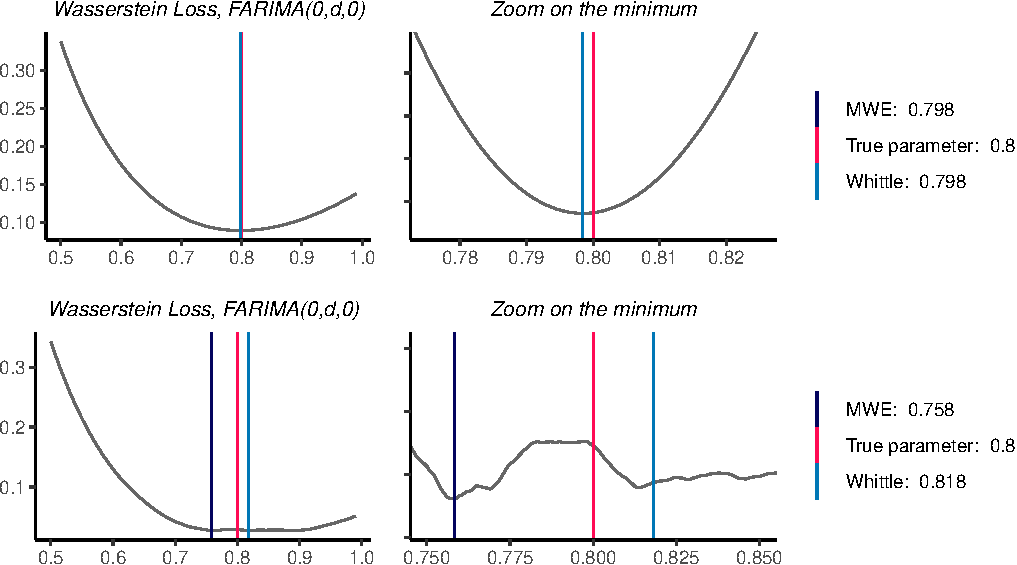
\includegraphics[width=0.6\linewidth]{Master_thesis_V2_files/figure-latex/wasserstein_farima-1} 

}

\caption{Wasserstein loss functions of two FARIMA(0,d,0) processes where H = 0.8 (d = 1.2). The sample size is 3001. The left column display the entire loss functions for all possible parameter values that a long-memory process can take (0.51 < H < 0.99). The right column is a zoom on the functions.}\label{fig:wasserstein_farima}
\end{figure}

Our first finding is that the computed distance might vary widely around
the true parameter value and its value depends heavily on the sample
simulated from an Exp(1), i.e.~observations \(z_1, ..., z_m\). As a
consequence, the estimated model parameter(s) \(\hat \theta_{MWE}\)
typically depend heavily on the random exponential variables generated
to conduct the optimization.

To illustrate the problem, on Figure \ref{fig:wasserstein_z} we continue
with the process used to plot the second line on Figure
\ref{fig:wasserstein_farima} and simply change the seed with which the
vector \(Z\) is generated. We remark that we are now dealing with a loss
function that is smooth and has a global minimum that is precisely the
true value of the parameter \(\theta^* = H = 0.8\). Therefore, we see
that by modifying the vector \(Z\), we can obtain a more appropriate
loss function. We find this aspect potentially problematic for numerical
optimization: by definition a random vector cannot be controlled and we
may obtain biased estimates simply because of the simulated variables
needed for the optimization procedure.

\begin{figure}[h]

{\centering 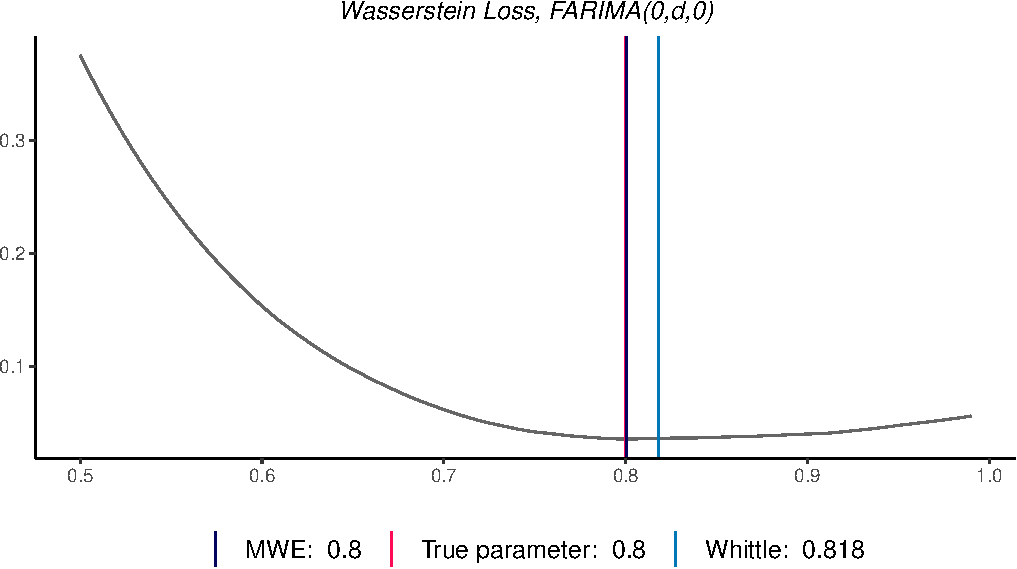
\includegraphics[width=0.55\linewidth]{Master_thesis_V2_files/figure-latex/wasserstein_z-1} 

}

\caption{Wasserstein loss function of the FARIMA(0,d,0) process (bottom one) of Figure 1 computed with another random vector.}\label{fig:wasserstein_z}
\end{figure}

In order to get a better overview of the behavior of the MWE when the
vector \(Z\) changes, we compute \(k = 200\) times
\(\hat \theta^*_{MWE}\) for a given process of size \(n = 3001\). Then,
we plot the results on Figure \ref{fig:MWE_n}. We can observe that, even
for large sample size, the estimated parameter depends heavily on the
random vector \(Z\). Nevertheless, the mean remains relatively close to
the true value.

\begin{figure}[h]

{\centering 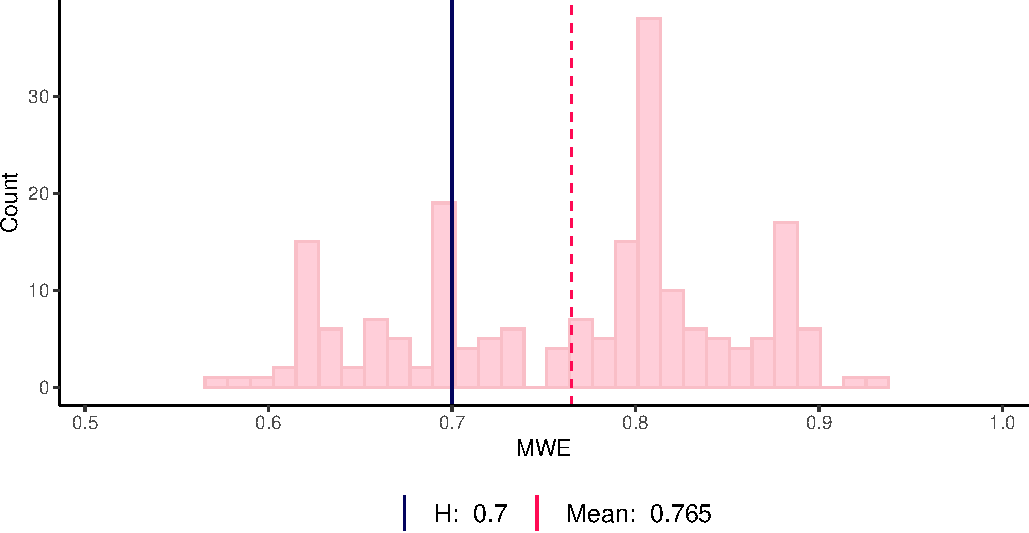
\includegraphics[width=0.6\linewidth]{Master_thesis_V2_files/figure-latex/MWE_n-1} 

}

\caption{We simulate 200 vectors following an exponential distribution and then compute the MWE of a FARIMA(0,d,0) process with n = 3001. The blue line is the true parameter H = 0.7 value and the red dashed line is the mean of the MWE.}\label{fig:MWE_n}
\end{figure}

To cope with this problem of dependence between the random vector \(Z\)
and the parameter estimate, we are going to explore two options.

\hypertarget{mean-of-minimum-wasserstein-estimators}{%
\subsubsection{Mean of Minimum Wasserstein
Estimators}\label{mean-of-minimum-wasserstein-estimators}}

Option A: for the simulated times series, we generate several
exponential random variables and stack them in vectors. Then, we
estimate the model parameter for each of the simulated vector and report
the mean of the estimated parameter.

For illustration, based on the same process than in Figure
\ref{fig:MWE_n} with \(n = 3001\), we generate
\(k = 10, 20 , 50, 100 , 200, 500, 1000\) random vectors, estimate the
\(k\) parameters and then report the mean. Thus, the mean becomes our
estimator and we note it \(\hat \theta^*_{MMWE}\). The results are
listed in Table \ref{tab:MWE_k}. As \(k\) increases, the average becomes
progressively closer to the true parameter.

\begin{table}[h]
\centering
\begin{tabular}{|c|c|c|c|c|c|c|c|c|}
\hline
$k$ &  1 & 10   & 20    & 50    & 100   & 200   & 500   & 1000 \\
\hline
$\hat \theta^*_{MMWE}$ & 0.807 & 0.73 & 0.727 & 0.726 & 0.721 & 0.719 & 0.714 & 0.714 \\
\hline
\end{tabular}
\caption{Mean of the minimum Wasserstein estimators for a FARIMA($0,d,0$) of size $n = 3001$ by varying the value of $k$, i.e. the number of exponential random vectors generated. The true value is 0.7.}
\label{tab:MWE_k}
\end{table}

\hypertarget{minimum-semidiscrete-wasserstein-estimator}{%
\subsubsection{Minimum Semidiscrete Wasserstein
Estimator}\label{minimum-semidiscrete-wasserstein-estimator}}

Option B: instead of using the empirical cumulative distribution
function (c.d.f) of exponential random variables generated from a
computer, we plan to use the c.d.f of exponential variables with rate
one for the SPOs, namely \(F(x)=1-e^{-x}\). Therefore, the Wasserstein
distance becomes:

\begin{equation}
\int_\mathcal{X}\left|\hat F(x)- (1 - e^{-x})\right| \mathrm{d} x 
\end{equation}

where \(\hat F(x) = \frac{1}{m} \sum_{j=1}^{m} 1_{X_{j} \leq x}\) and
\(x_j\) are the SPOs of a process. To compute this distance, we replace
\(\hat F_\mu(z) = \frac{1}{m}\sum_{j=1}^{m} \mathbf{1}_{Z_{j} \leq z}\)
by \(F_\mu = 1 - e^{-x}\). We use a trapezoidal integration to
approximate the integral. Thanks to this second option, there is no
longer randomness in our process estimation. The corresponding loss
functions for two FARIMA(\(0,d,0\)) processes using this method are
showed in Figure \ref{fig:semi_wass}

\begin{figure}

{\centering 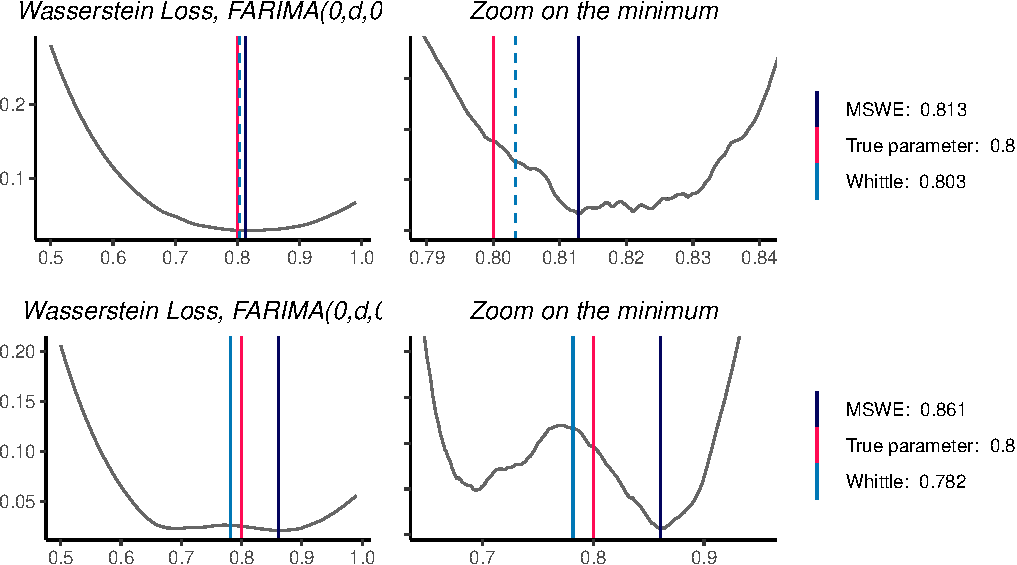
\includegraphics[width=0.6\linewidth]{Master_thesis_V2_files/figure-latex/semi_wass-1} 

}

\caption{Semidiscrete Wasserstein loss functions for two FARIMA(0,d,0) processes. The sample size is 3001 and the true parameter value is 0.8.}\label{fig:semi_wass}
\end{figure}

Still, another problem persists. The Wasserstein loss, even for large
sample size, is often not well-shaped (i.e smooth and concave): it may
contain several local minima (see e.g.~Figure
\ref{fig:wasserstein_farima}). This concern leads to biased estimates
with large variance. It should also be noted that the loss shape
degenerates even more when n decreases (see Figure
\ref{fig:small_sample}). So far, we are not able to explain why there is
such diversity in the shape of the loss functions.

\begin{figure}

{\centering 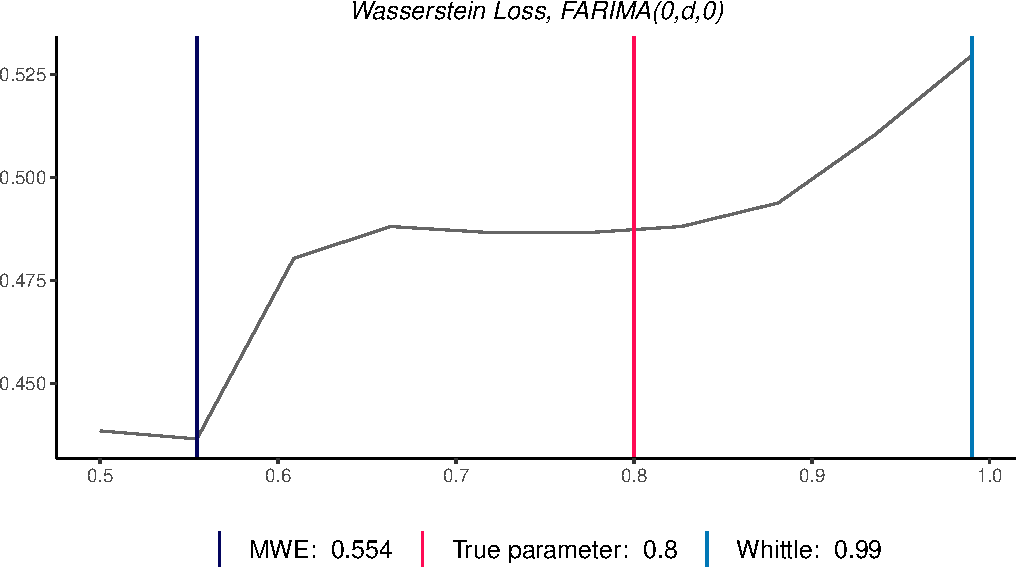
\includegraphics[width=0.5\linewidth]{Master_thesis_V2_files/figure-latex/small_sample-1} 

}

\caption{Wasserstein loss function of a FARIMA(0,d,0) process with sample size equal to 51.}\label{fig:small_sample}
\end{figure}

\hypertarget{minimum-weighted-wasserstein-estimator}{%
\subsubsection{Minimum Weighted Wasserstein
Estimator}\label{minimum-weighted-wasserstein-estimator}}

After searching a way to fix this problem, we found that by putting some
weights in the loss function defined by the Wasserstein distance, we
obtain a much more regular optimization problem. Therefore, we seek the
parameter that minimizes

\begin{equation}
\mathcal{W}_{1}(\mu, \nu)=\int_{\mathbb{R}}\left|F_{\mu}(t)-F_{\nu}(t)\right| d t
\end{equation}

where the empirical cumulative distribution of the SPOs is
\(\hat F_\nu(x)=\sum_{i=1}^{m} w_{j} 1\left\{X_{i} \leq x\right\}\) and
the weights \(w_j\) are

\begin{equation}
w_j = \frac{\frac{I(\lambda_j)}{f(\lambda_j; \theta)}}{\sum^m_{j = 1}\frac{I(\lambda_j)}{f(\lambda_j; \theta)}}.
\label{eq:weights}
\end{equation}

We call the estimator minimizing this new distance our minimum weighted
Wasserstein estimator (MWWE) \(\theta^*_{MWWE}\).

The employment conditions of R packages to calculate the distances used
in this thesis required that the weights sum to \(1\) and that are
comprised between \(0\) and \(1\). Therefore, our first intuition is to
use the weights proposed in Eq. \ref{eq:weights}. Intuitively, these
weights give more leverage to extreme values while computing the
Wasserstein distance.

Figure \ref{fig:weighted_wasserstein} shows the same process and vector
\(Z\) as Figure \ref{fig:wasserstein_farima} but applies the weights to
calculate our weighted Wasserstein distance. We can observe that the
weighted Wasserstein loss function is immediately smoother and contains
a minimum which is even closer to the true parameter than the Whittle's
estimator.

\begin{figure}

{\centering 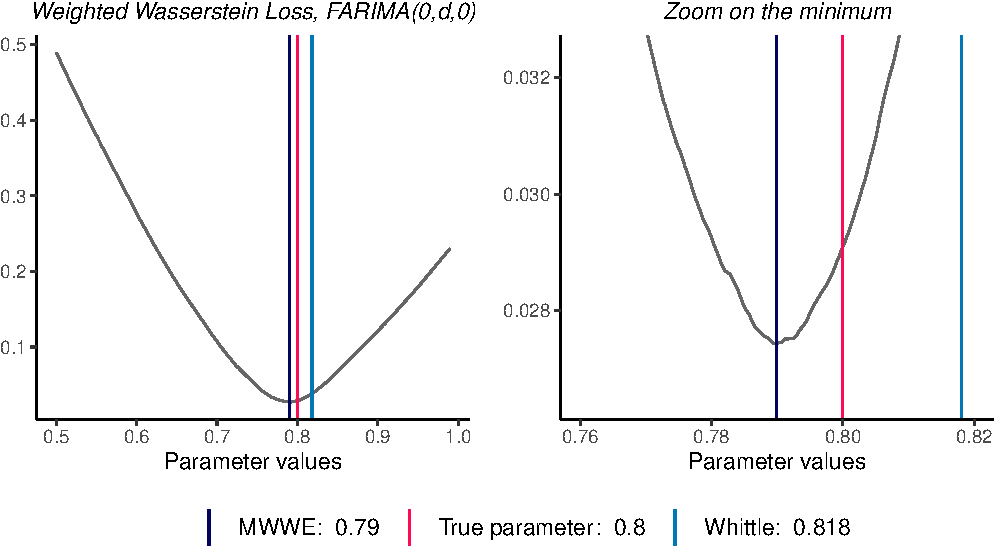
\includegraphics[width=0.6\linewidth]{Master_thesis_V2_files/figure-latex/weighted_wasserstein-1} 

}

\caption{Weighted Wasserstein loss function of the FARIMA(0,d,0) process on Figure 1 (bottom).}\label{fig:weighted_wasserstein}
\end{figure}

It is important to note that the weights applied here are not optimal
and, therefore, this question remains open and subject to further
analysis. However, the weights presented in this section work well
especially for ARMA(\(p,q\)) processes as illustrated on Figure
\ref{fig:wass_ar1_weighted}. The shape of the loss function using the
weighted Wasserstein estimator suggests that we could obtain an
estimator with small variance. We could, for instance, implement a
minimum expected Wasserstein estimator defined by
\protect\hyperlink{ref-bernton2019parameter}{Bernton et al.}
(\protect\hyperlink{ref-bernton2019parameter}{2019}). This option could
be investigated in future research.

\begin{figure}

{\centering 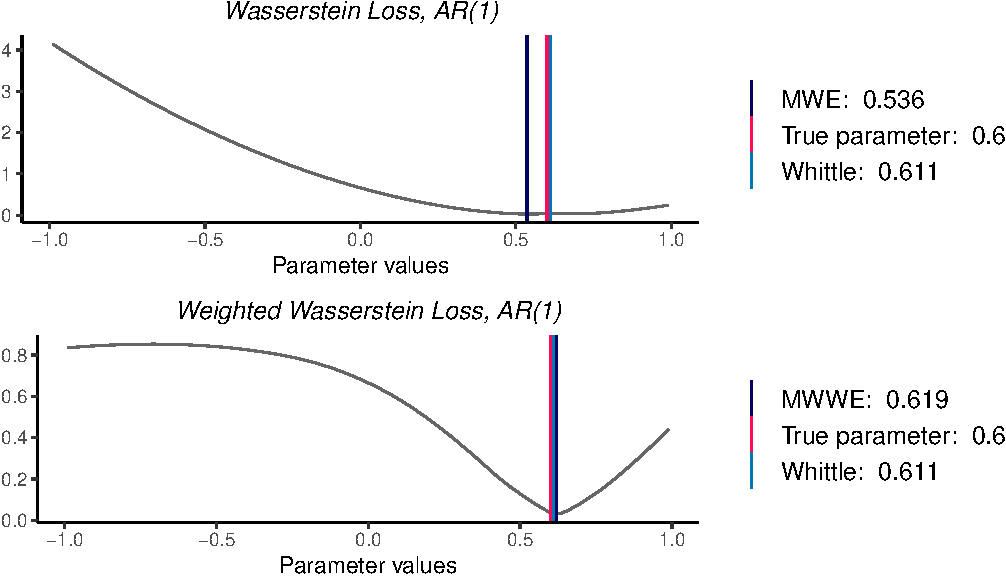
\includegraphics[width=0.55\linewidth]{Master_thesis_V2_files/figure-latex/wass_ar1_weighted-1} 

}

\caption{Wasserstein loss function and weighted Wasserstein loss function of a Gaussian AR(1) process. The sample size is 3001 and the true parameter is 0.6.}\label{fig:wass_ar1_weighted}
\end{figure}

\hypertarget{minimum-sinkhorn-estimator}{%
\subsubsection{Minimum Sinkhorn
Estimator}\label{minimum-sinkhorn-estimator}}

A second idea is to employ the Sinkhorn divergence (see Eq.
\ref{eq:sink}) to estimate our parameter based on
\protect\hyperlink{ref-cuturi2013sinkhorn}{Cuturi}
(\protect\hyperlink{ref-cuturi2013sinkhorn}{2013}). The regularization
term should make the loss function smoother. On Figure
\ref{fig:sinkhorn}, we compare the loss function when we employ the
Wasserstein distance or the Sinkhorn divergence to estimate our
parameter. Indeed, we end up with a smooth and concave function. The
reached minimum is very close to the true value. A good property with
the Sinkhorn divergence is that it remains smooth even for a very small
sample size.

\begin{figure}

{\centering 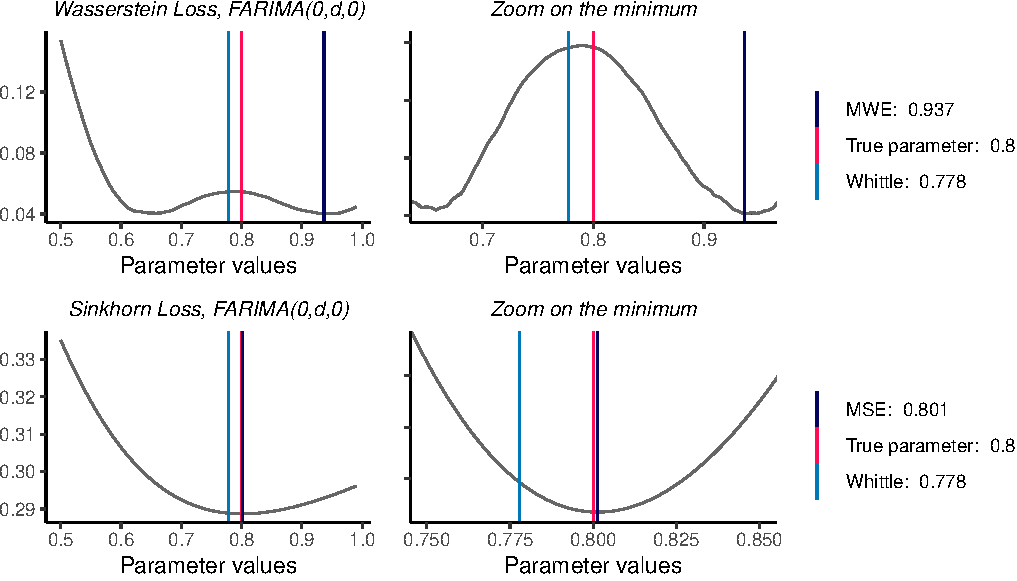
\includegraphics[width=0.65\linewidth]{Master_thesis_V2_files/figure-latex/sinkhorn-1} 

}

\caption{Top: Wasserstein loss function of a FARIMA(0,d,0) process. Bottom: Sinkhorn loss function of the same process. The sample size is 1801.}\label{fig:sinkhorn}
\end{figure}

Following this, we are confronted to an important choice: which values
to select for \(\lambda\)? As a reminder, when \(\lambda\) is very
small, the Sinkhorn divergence approximates the Wasserstein distance. In
order to choose the optimal lambda we suggest to implement classical
machine learning techniques to perform model selection such as cross
validation, leave-one-out, etc. For more information see for example
\protect\hyperlink{ref-friedman2001elements}{Friedman et al.}
(\protect\hyperlink{ref-friedman2001elements}{2001}) Chapter 7.

To illustrate, we randomly divide a time series into \(2\) groups
\(C_1 \ (80\%), C_2 \ (20\%)\) also called folds. We treat the first
group as train and the second group as validation/test. For a selection
of \(\lambda\), we estimate our parameter, the minimum Sinkhorn
estimator (MSKE), on the train set and then use the corresponding
\(\hat \theta_{MSKE}\) to predict the time data of our test set. For
simplicity, we demonstrate the procedure with an AR(1) process,
\(Y_t = \phi_1 Y_{t-1} + \epsilon_t\) where \(\epsilon_t \sim N(0,1)\)
and \(\theta^* = \phi_1 = 0.6\). After estimating the parameter thanks
to the train set, we substitute its value in
\(\hat \epsilon_t = Y_t - \hat \theta^*_{MSKE} Y_{t-1}\) where
\(t = 2, ..., l\). \(l\) is the length of the testing vector and depends
on which ratios we choose to split our time process \({Y_t}\) in our
case \(80\% - 20\%\). Then, we use the predictions of the error terms to
compute the Mean Squared Error for a given \(\lambda\):

\[MSE_{\lambda} \textit{ of the test set} = \frac{1}{l}\sum_{t = 2}^l \hat \epsilon_t^2 = \frac{1}{l} \sum_{t = 2}^l (Y_t - \hat \theta^*_{MSKE} Y_{i-t})^2\]

We repeat this method for several lambda values and plot the results on
Figure \ref{fig:SH_CV}. The minimum testing error is achieved when
\(\lambda = 0.1\) given an estimate
\(\hat \theta^*_{MSKE_{\lambda = 0.1}} = 0.572\) which is close to the
true parameter value \(\theta^* = 0.6\).

\begin{figure}

{\centering 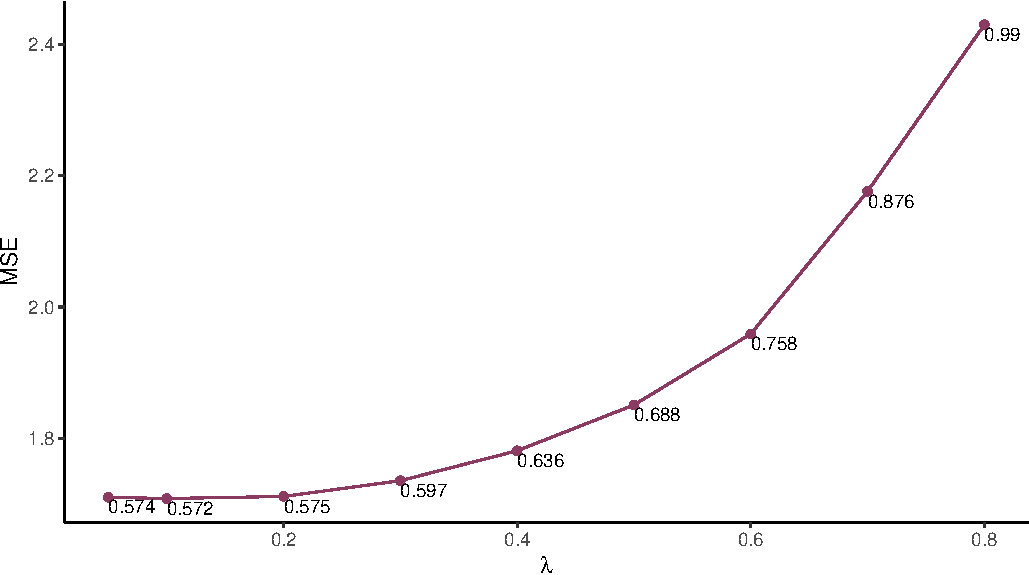
\includegraphics[width=0.55\linewidth]{Master_thesis_V2_files/figure-latex/SH_CV-1} 

}

\caption{Testing MSE vs lambda values for an AR(1) process. The sample size is  4001 and the true parameter value is 0.6. For this process, the minimum MSE is achieved when lambda = 0.1.}\label{fig:SH_CV}
\end{figure}

\hypertarget{results}{%
\section{Results}\label{results}}

\hypertarget{monte-carlo-simulations}{%
\subsection{Monte Carlo Simulations}\label{monte-carlo-simulations}}

Our criterion for evaluating the performance of each of the estimators
is, as it is often the case in machine learning, the Mean Squared Error
(\(MSE\))

\[MSE(\hat \theta^*, \theta^*) =  \frac{1}{mt}\sum^{mt}(\hat \theta^* - \theta^*)^2 \approx \operatorname{Var}(\hat{\theta^*})+\operatorname{Bias}^{2}(\hat{\theta^*})\]

where \(mt\) is the number of Monte Carlo simulations, i.e.~the number
of simulated processes. The MSE represents the bias-variance trade-off
which typically emerges in statistics when it comes to model selection.

\hypertarget{long-memory-process}{%
\subsubsection{Long-memory Process}\label{long-memory-process}}

Firstly, we simulate \(mt = 400\) stationary FARIMA(\(0,d,0\)) processes
of size \(n = 3201\) and \(H = 0.8 \ (d = 0.3)\) according to

\[(1-L)^{0.3}Y_t = \epsilon_t.\]

For each process, we compute the Whittle's estimator
\(\hat \theta^*_{WH}\), the minimum Wasserstein estimator
\(\hat \theta^*_{MWE}\), the mean of the minimum Wasserstein estimators
\(\hat \theta^*_{MMWE}\), the minimum semidiscrete Wasserstein estimator
\(\hat \theta^*_{MSWE}\), the minimum weighted Wasserstein estimator
\(\hat \theta^*_{MWWE, \ k}\) and the minimum Sinkhorn estimator
\(\hat \theta^*_{MSKE,\ \lambda}\). Figure \ref{fig:box_farima_400}
reports the results.

\begin{figure}

{\centering \includegraphics[width=0.75\linewidth]{/Users/manonfelix/OneDrive/Master thesis/Redaction/images/box_400_farima_gauss} 

}

\caption{Boxplots of all the estimators presented during this thesis. The sample size of the 400 simulated FARIMA(0,d,0) is 3201.}\label{fig:box_farima_400}
\end{figure}

We note that the minimum Wasserstein estimator has very high variance
due to the problems mentioned earlier. As expected, by using either the
mean of the minimum Wasserstein estimators or the minimum semidiscrete
Wasserstein estimator, we can reduce the variance. Our minimum weighted
Wasserstein estimator is similar to Whittle's estimator in terms of Mean
Squared Error. Indeed, both new estimators have small variance and no
bias. The density of these two estimators is in Figure
\ref{fig:density_long_gauss}. Both distributions are centered around the
true parameter and have similar shape. Nevertheless, the minimum
weighted Wasserstein estimator has larger tails, i.e larger variance.

The use of the Sinkhorn distance also seems promising but depends on the
\(\lambda\) parameter. When \(\lambda\) is equal to \(0.1\), the minimum
Sinkhorn estimator is well centered around the true parameter and has a
reasonable variance. Here, we do not choose \(\lambda\) by
cross-validation because of the time needed for computation. We compute
the Sinkhorn distance where the value of \(\lambda\) is determined in
advance. It is expected that by performing a selection of lambda
parameters we will obtain even better results.

\begin{figure}

{\centering \includegraphics[width=0.6\linewidth]{/Users/manonfelix/OneDrive/Master thesis/Redaction/images/density_long} 

}

\caption{Distribution of the Whittle's estimator and the weighted Wasserstein estimator estimated with the 400 simulations of Figure xx.}\label{fig:density_long_gauss}
\end{figure}

\begin{table}[h]
\centering
\begin{tabular}{|l|c|}
\hline
                      & $MSE(\hat \theta^*, \theta^*)$                \\ \hline
\textbf{Distribution} & \textbf{Gaussian}                    \\ \hline
$\hat \theta^*_{Whittle}$                   & 0.00021                                \\ \hline
$\hat \theta^*_{MWE}$                      & 0.00436                                \\ \hline
$\hat \theta^*_{MMWE, \ k = 50}$            & 0.00324                               \\ \hline
$\hat \theta^*_{MSWE}$                     & 0.00418                                \\ \hline
$\hat \theta^*_{MWWE}$                       & 0.00030                                \\ \hline
$\hat \theta^*_{MSKE, \ \lambda = 0.1}$      & 0.00061                               \\ \hline
$\hat \theta^*_{MSKE, \ \lambda = 0.3}$      & 0.00144                               \\ \hline
\end{tabular}
\caption{Mean Squared Errors of Figure 10.}
\label{tab:farima_mse_gaussian}
\end{table}

\hypertarget{heavy-tailed-distribution}{%
\subsubsection{Heavy-tailed
Distribution}\label{heavy-tailed-distribution}}

\protect\hyperlink{ref-mikosch1995parameter}{Mikosch et al.}
(\protect\hyperlink{ref-mikosch1995parameter}{1995}) showed that the
fatter the tails of the innovation distributions, the faster the
Whittle's estimator converges to the true parameter value. Regarding the
Wasserstein loss function, it becomes smooth and concave when the error
distribution is heavy-tailed (see Figure \ref{fig:student_t}), even for
small sample sizes. Therefore, the Whittle's estimator and the MWE are
usually very close in value.

\begin{figure}

{\centering 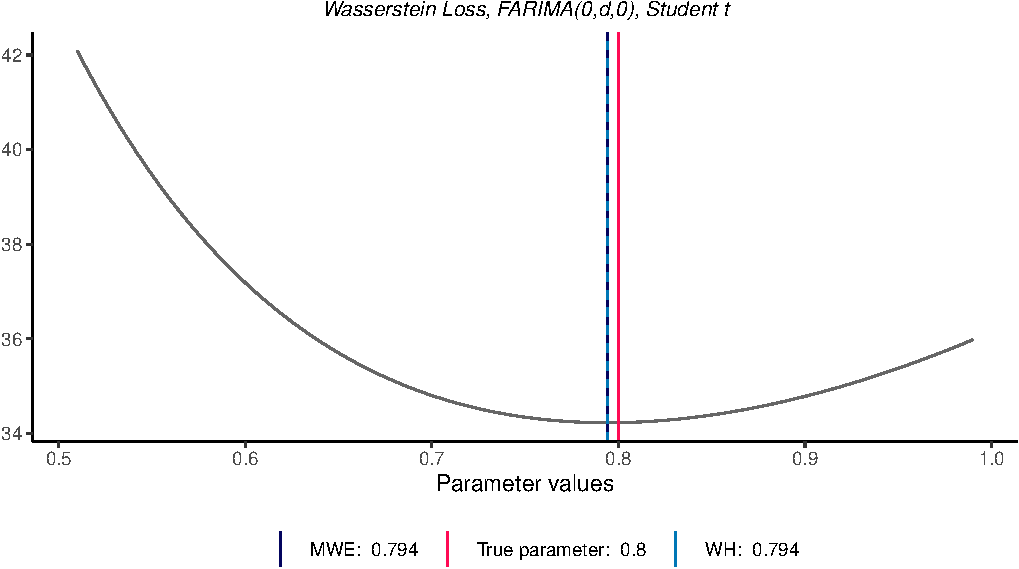
\includegraphics[width=0.6\linewidth]{Master_thesis_V2_files/figure-latex/student_t-1} 

}

\caption{Wasserstein loss function of a FARIMA(0,d,0) process distributed according to a Student t distribution with degree of freedom equal to 2. The sample size is equal to 3001.}\label{fig:student_t}
\end{figure}

We simulate again \(mt = 400\) FARIMA(0,d,0) processes with a Student t
underlying distribution with degree of freedom equal to 2. On Figure
\ref{fig:box_farima_student}, we note that all estimators (apart from
those based on the Sinkhorn distance) have a considerably smaller
variance than when the process is Gaussian and, consequently, a smaller
MSE (see Table \ref{tab:FARIMA_heavy_MSE}).

\begin{figure}

{\centering \includegraphics[width=0.65\linewidth]{/Users/manonfelix/OneDrive/Master thesis/Redaction/images/box_student_400_farima} 

}

\caption{Boxplots of all the estimators presented during this thesis. The sample size of the 200 simulated FARIMA(0,d,0) is 3201 and the underlying distribution is a Student t with degree of freedom equal to 2.}\label{fig:box_farima_student}
\end{figure}

\hypertarget{skewed-and-heavy-tailed-distribution}{%
\subsubsection{Skewed and Heavy-tailed
Distribution}\label{skewed-and-heavy-tailed-distribution}}

Let us now focus on the case where the distribution of the innovation
terms remains heavy-tailed but on top of that skewed. The skew t
distribution was recently developed by
\protect\hyperlink{ref-azzalini2003distributions}{Azzalini and
Capitanio} (\protect\hyperlink{ref-azzalini2003distributions}{2003}). It
is related to a standard skew normal random variable \(T\) and a random
variable \(M\) following a chi-squared distribution with \(\nu\) degree
of freedom by the equation:

\[R=\frac{T}{\sqrt{\frac{M}{\nu}}}.\]

Then the linear transformation \(X=\mu+\sigma R\) has a skew-t
distribution with parameters \(\mu, \sigma, \alpha\), and \(\nu\) and
the corresponding notation \(S T(\mu = 0, \sigma = 1, \gamma, \nu)\) to
denote the skew t random variable \(X\). For example, we consider the
underlying distribution of the process as a skew t distribution with
degree of freedom equal to 2 and skewness parameter \(\gamma\) equal to
4. The corresponding density function is represented on Figure
\ref{fig:skewt_density}).

\begin{figure}

{\centering 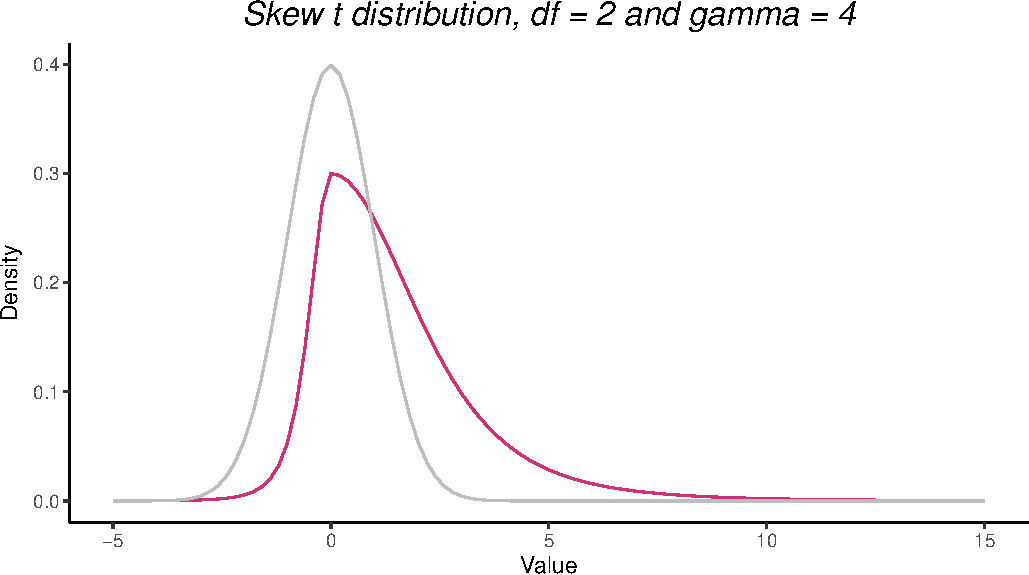
\includegraphics[width=0.5\linewidth]{Master_thesis_V2_files/figure-latex/skewt_density-1} 

}

\caption{Skew t distribution with degree of freedom = 2 and gamma = 4 (pink) and standard normal distribution (grey).}\label{fig:skewt_density}
\end{figure}

On Figure \ref{fig:skew_t}, we compute the Wasserstein loss function in
the case of skew t distributed FARIMA(0,d,0) process. The loss remains
smooth and concave, as it is the case for a Student t underlying
distribution, but the parameter minimizing the loss function has a much
larger value than the true parameter (\(0.945 > 0.8\)). The same effect
occurs for the Whittle's estimator, we also overestimate the parameter
value (see Figure \ref{fig:skew_t}).

\begin{figure}

{\centering 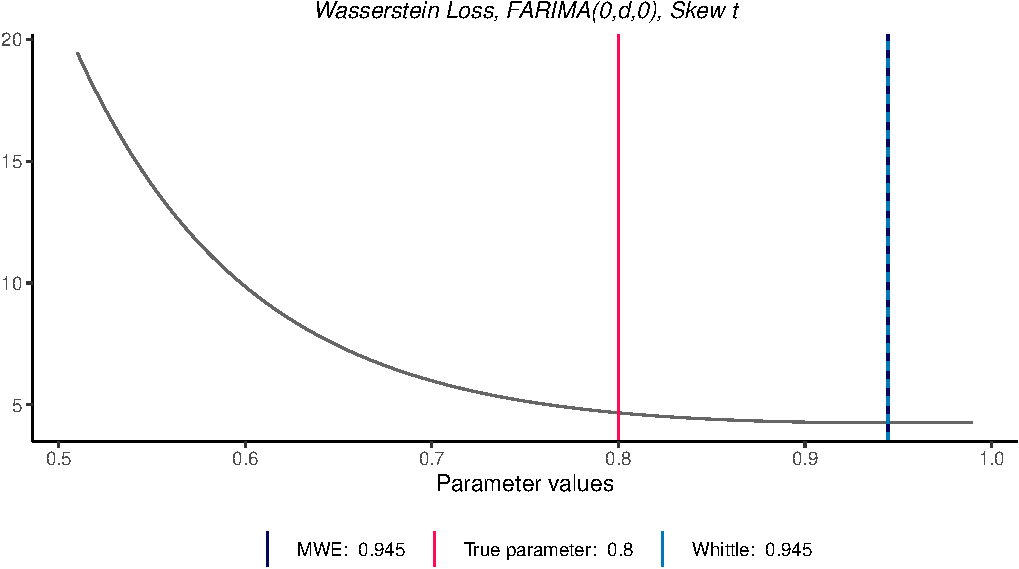
\includegraphics[width=0.5\linewidth]{Master_thesis_V2_files/figure-latex/skew_t-1} 

}

\caption{Wasserstein loss function of a FARIMA(0,d,0) process distributed according to a skew t distribution with degree of freedom = 4 and gamma = 2. The sample size is equal to 3001.}\label{fig:skew_t}
\end{figure}

We compare all the estimators when the underlying distribution is a skew
t on Figure \ref{fig:box_farima_skewt}. All estimators are biased in the
sense they overestimate the value of the parameter. Some are more biased
than others and curiously the minimum Wasserstein estimator is the least
biased but it has a greater variance than others estimators. Regarding
the Mean Squared Error values listed in Table
\ref{tab:FARIMA_heavy_MSE}, all our new estimators surpass the Whittle's
estimator except the minimum weighted Wasserstein estimator. This gain
in terms of MSE is mainly due to a gain in bias since most estimators
have a similar variance to Whittle's. The estimator with the smallest
MSE is the one obtained by means of the Sinkhorn distance when
\(\lambda = 0.1\).

In order to verify that this bias does not come from the fact that the
error distribution is skewed we also simulated processes coming from a
skew normal distribution (left and right skewed). Then, we reproduced
the same boxplots and what we observe is that there is no bias. All
these results are available on the Github link mentioned at the
beginning of this thesis.

\begin{figure}[h]

{\centering \includegraphics[width=0.6\linewidth]{/Users/manonfelix/OneDrive/Master thesis/Redaction/images/skewt_box_400} 

}

\caption{Boxplots of all the estimators presented during this thesis. The sample size of the 200 simulated FARIMA(0,d,0) is 3201 and the underlying distribution is a skew t with df = 4 and gamma = 2.}\label{fig:box_farima_skewt}
\end{figure}

\begin{table}[h]
\centering
\begin{tabular}{|l|c|c|}
\hline
          & $MSE(\hat \theta^*, \theta^*)$   & $MSE(\hat \theta^*, \theta^*)$  \\ \hline
\textbf{Distribution} & \textbf{Student t}  & \textbf{Skew t}     \\ \hline
$\hat \theta^*_{Whittle}$                & 0.000295               & 0.023688             \\ \hline
$\hat \theta^*_{MWE}$                    & 0.000565               & 0.012266              \\ \hline
$\hat \theta^*_{MMWE, \ k = 50}$            & 0.000294              & 0.021146              \\ \hline
$\hat \theta^*_{MSWE}$                    & 0.000305               & 0.021387              \\ \hline
$\hat \theta^*_{MWWE}$                    & 0.000354               & 0.030284              \\ \hline
$\hat \theta^*_{MSKE, \ \lambda = 0.1}$                & 0.000653               & 0.013515              \\ \hline
$\hat \theta^*_{MSKE, \ \lambda = 0.3}$                 & 0.001260               & 0.020946             \\ \hline
\end{tabular}
\caption{Mean Squared Error of Figure 13 and 16.}
\label{tab:FARIMA_heavy_MSE}
\end{table}

\pagebreak

\hypertarget{additive-outliers}{%
\subsubsection{Additive Outliers}\label{additive-outliers}}

In the presence of contamination in the time series (e.g.~additive
outliers). For example, in the case of Gaussian FARIMA(0, d, 0) some
of our estimators (in particular, the ones based on weighted Wasserstein
distance and/or on the Sinkhorn divergence) seem to overperform
Whittle's estimator in terms of MSE. To demonstrate this propriety we
simulate \(mt = 200\) FARIMA(\(0,d,0\)) contaminated by occasional
isolated outliers. The processes \(\{Y_t\}\) are distributed according
to

\[Y_{t}=\left(1-W_{t}\right) X_{t}+W_{t}\left(c \cdot V_{t}\right)\]
where \(W_t \sim Bern(p)\), \(V_t \sim t_2\) and c = 10. 

In Table
\ref{tab:outliers}, we report the ratio between the MSE of the Whittle's
estimator and the minimum weighted Wasserstein estimator for different
values of \(p = 0, 0.001, 0.01, 0.05\) (when \(p = 0\) the process is not contaminated by outliers). The results suggest that when the time series is
contaminated, the minimum weighted Wasserstein estimator overperform the Whittle's estimator in terms of
MSE since as soon as we introduce noise the ratio becomes greater than 1.  

\begin{table}[h]
\centering
\begin{tabular}{|c|c|c|c|c|}
\hline
p  &  0  & 0.001   & 0.01    & 0.05 \\
\hline
ratio  & 0.682 & 1.208 & 1.105 & 1.012 \\
\hline
\end{tabular}
\caption{Mean Squared Error of the Whittle's estimator divided by the Mean Squared Error of the minimum weighted Wasserstein estimator. The number of simulated time series is equal to 200 with sample size equal to 3001.}
\label{tab:outliers}
\end{table}

\hypertarget{short-memory-process}{%
\subsubsection{Short-memory Process}\label{short-memory-process}}

We also aim to demonstrate the performance of our estimators for
short-memory processes. To do this, we simulate \(mt = 400\)
auto-regressive processes of order 2 according to:

\[Y_t = 0.75 Y_{t-1} - 0.25Y_{t-2} + \epsilon_t.\]

The processes are stationary since the three stationary conditions are
met:

\begin{enumerate}
\def\labelenumi{\arabic{enumi}.}
\tightlist
\item
  \(\phi_{2}<1+\phi_{1}\)
\item
  \(\phi_{2}<1-\phi_{1}\)
\item
  \(\phi_{2}>-1\)
\end{enumerate}

where \(\phi_1 = 0.75\) and \(\phi_2 = -0.25\).

We cannot include the Sinkhorn divergence in our comparison because the
function used on R requires too much time to calculate this divergence
and fails to converge. The results when
\(\theta^* \subset \mathbb{R}^2\) are on Figure \ref{fig:box_ar2} with
corresponding MSE in Table \ref{tab:AR2_mse_table}. Again, we consider
several distributions for \(\epsilon_t\):
\(\epsilon_t \sim N(0,1), \epsilon_t \sim t_2\) and
\(\epsilon_t \sim S T(\mu = 0, \sigma = 1, \gamma = 2, \nu = 4)\) (Gaussian, Student t and skew t).

\begin{center}\includegraphics[width=0.6\linewidth]{/Users/manonfelix/OneDrive/Master thesis/Redaction/images/box_ar2_gauss_400} \end{center}

\begin{center}\includegraphics[width=0.6\linewidth]{/Users/manonfelix/OneDrive/Master thesis/Redaction/images/box_ar2_student_400} \end{center}

\begin{figure}

{\centering \includegraphics[width=0.6\linewidth]{/Users/manonfelix/OneDrive/Master thesis/Redaction/images/box_ar2_skew_400} 

}

\caption{Boxplots of the Whittle's estimator, MWE, MSWE, MMWE, MWWE for 400 AR(2) processes. The innovation terms densities are (in the order of apparition): Gaussian, Student t, Skew t. The left column is the first parameter (0.75) of the process, the right one is for the second parameter (-0.25).}\label{fig:box_ar2}
\end{figure}

When the process is Gaussian, the MSE of the minimum weighted
Wasserstein estimator is similar to Whittle's estimator. The other
estimators have larger variance than Whittle's. As observed for
processes with long-memory, when the tails of the error distributions
are wider than those of the normal distribution, the minimum Wasserstein
estimator converges to Whittle's estimator in terms of bias and
variance. In the case of Student t innovation term, all estimators are
relatively similar in terms of MSE (bias - variance). On the other hand,
contrary to long-memory processes, we observe that the fact that the
underlying distribution are skewed or not is not relevant during the
estimation procedure and the estimator do not overestimate the true
parameter. Indeed, the results for the Student t and the skew t
distribution are very close.

\begin{table}[h]
\centering
\begin{tabular}{|l|c|c|c|c|c|c|}
\hline
$MSE(\hat \theta^*, \theta^* = \phi_i)$        & $\phi_1$           & $\phi_2$          & $\phi_1$           & $\phi_2$           & $\phi_1$          & $\phi_2$         \\ \hline
\textbf{Distribution} & \multicolumn{2}{l|}{\textbf{Gaussian}} & \multicolumn{2}{l|}{\textbf{Student t}} & \multicolumn{2}{l|}{\textbf{Skew t}} \\ \hline
$\hat \theta^*_{Whittle}$                & 0.00028              & 0.00031             & 0.00027              & 0.00029              & 0.00033             & 0.00029            \\ \hline
$\hat \theta^*_{MWE}$                   & 0.00512              & 0.00703             & 0.00070             & 0.00066              & 0.00134             & 0.00143            \\ \hline
$\hat \theta^*_{MMWE, \ k = 50}$          & 0.00313              & 0.00317             & 0.00033              & 0.00038              & 0.00045             & 0.00044            \\ \hline
$\hat \theta^*_{MSWE}$                  & 0.00397              & 0.00407             & 0.00030              & 0.00033              & 0.00033             & 0.00030            \\ \hline
$\hat \theta^*_{MWWE}$                  & 0.00038              & 0.00045             & 0.00035              & 0.00038             & 0.00047             & 0.00038            \\ \hline
\end{tabular}
\caption{Mean Squared Error of Figure 17.}
\label{tab:AR2_mse_table}
\end{table}

\hypertarget{conclusion}{%
\section{Conclusion}\label{conclusion}}

To conclude, we introduce, in this thesis, five new estimators that are
based on minimum distance estimation. Our results suggest that we can
outperform the state-of-the art estimation procedure when we are dealing
with long-memory processes that have skewed underlying distributions.
Moreover, it seems that our minimum weighted Wasserstein estimator can
also be more efficient when the process is contaminated by occasional
outliers. In the case of short memory processes, we have similar results
to Whittle's estimator in terms of MSE. Through this thesis, we open the
possibility for further research. Indeed, the weights are certainly not
optimal and therefore would be subject to further investigation. As well
as the choice of the regularization parameter when using the Sinkhorn
divergence. The shape of the Wasserstein loss function and why the
estimation procedure behaves better for certain vector \(Z_j\) also
remains an opened question. We can also extend our research to other
distances such as the energy distance:

\[D^{2}(F, G)=2 \int_{-\infty}^{\infty}(F(t)-G(t))^{2} \mathrm{~d} t.\]
Another important step is to compute the theory surrounding these
estimators (consistency, robustness, etc.). To sum up, our results are
promising and open the possibility of further researches.

\newpage

\hypertarget{references}{%
\section*{References}\label{references}}
\addcontentsline{toc}{section}{References}

\hypertarget{refs}{}
\begin{CSLReferences}{1}{0}
\leavevmode\hypertarget{ref-ambrosio2013user}{}%
Ambrosio, Luigi, and Nicola Gigli. 2013. {``A User's Guide to Optimal
Transport.''} In \emph{Modelling and Optimisation of Flows on Networks},
1--155. Springer.

\leavevmode\hypertarget{ref-arjovsky2017wasserstein}{}%
Arjovsky, Martin, Soumith Chintala, and Léon Bottou. 2017.
{``Wasserstein Generative Adversarial Networks.''} In
\emph{International Conference on Machine Learning}, 214--23. PMLR.

\leavevmode\hypertarget{ref-azzalini2003distributions}{}%
Azzalini, Adelchi, and Antonella Capitanio. 2003. {``Distributions
Generated by Perturbation of Symmetry with Emphasis on a Multivariate
Skew t-Distribution.''} \emph{Journal of the Royal Statistical Society:
Series B (Statistical Methodology)} 65 (2): 367--89.

\leavevmode\hypertarget{ref-bassetti2006minimum}{}%
Bassetti, Federico, Antonella Bodini, and Eugenio Regazzini. 2006. {``On
Minimum Kantorovich Distance Estimators.''} \emph{Statistics \&
Probability Letters} 76 (12): 1298--1302.

\leavevmode\hypertarget{ref-basu2019statistical}{}%
Basu, Ayanendranath, Hiroyuki Shioya, and Chanseok Park. 2019.
\emph{Statistical Inference: The Minimum Distance Approach}. Chapman;
Hall/CRC.

\leavevmode\hypertarget{ref-beran1994statistics}{}%
Beran, Jan. 1994. \emph{Statistics for Long-Memory Processes}. Vol. 61.
CRC press.

\leavevmode\hypertarget{ref-bernton2019parameter}{}%
Bernton, Espen, Pierre E Jacob, Mathieu Gerber, and Christian P Robert.
2019. {``On Parameter Estimation with the Wasserstein Distance.''}
\emph{Information and Inference: A Journal of the IMA} 8 (4): 657--76.


\leavevmode\hypertarget{ref-brillinger2001time}{}%
Brillinger, David R. 2001. \emph{Time Series: Data Analysis and Theory}.
SIAM.

\leavevmode\hypertarget{ref-cuturi2013sinkhorn}{}%
Cuturi, Marco. 2013. {``Sinkhorn Distances: Lightspeed Computation of
Optimal Transport.''} \emph{Advances in Neural Information Processing
Systems} 26: 2292--2300.

\leavevmode\hypertarget{ref-friedman2001elements}{}%
Friedman, Jerome, Trevor Hastie, Robert Tibshirani, and others. 2001.
\emph{The Elements of Statistical Learning}. Vol. 1. 10. Springer series
in statistics New York.

\leavevmode\hypertarget{ref-kantorovich1942translocation}{}%
Kantorovich, Leonid V. 1942. {``On the Translocation of Masses.''} In
\emph{Dokl. Akad. Nauk. USSR (NS)}, 37:199--201.

\leavevmode\hypertarget{ref-kolouri2017optimal}{}%
Kolouri, Soheil, Se Rim Park, Matthew Thorpe, Dejan Slepcev, and Gustavo
K Rohde. 2017. {``Optimal Mass Transport: Signal Processing and
Machine-Learning Applications.''} \emph{IEEE Signal Processing Magazine}
34 (4): 43--59.

\leavevmode\hypertarget{ref-mikosch1995parameter}{}%
Mikosch, Thomas, Tamar Gadrich, Claudia Kluppelberg, and Robert J Adler.
1995. {``Parameter Estimation for ARMA Models with Infinite Variance
Innovations.''} \emph{The Annals of Statistics}, 305--26.

\leavevmode\hypertarget{ref-monge1781memoire}{}%
Monge, Gaspard. 1781. {``M{é}moire Sur La Th{é}orie Des d{é}blais Et Des
Remblais.''} \emph{Histoire de l'Acad{é}mie Royale Des Sciences de
Paris}.

\leavevmode\hypertarget{ref-ni2020conditional}{}%
Ni, Hao, Lukasz Szpruch, Magnus Wiese, Shujian Liao, and Baoren Xiao.
2020. {``Conditional Sig-Wasserstein GANs for Time Series Generation.''}
\emph{arXiv Preprint arXiv:2006.05421}.

\leavevmode\hypertarget{ref-panaretos2020invitation}{}%
Panaretos, Victor M, and Yoav Zemel. 2020. \emph{An Invitation to
Statistics in Wasserstein Space}. Springer Nature.

\leavevmode\hypertarget{ref-peyre2019computational}{}%
Peyré, Gabriel, Marco Cuturi, and others. 2019. {``Computational Optimal
Transport: With Applications to Data Science.''} \emph{Foundations and
Trends in Machine Learning} 11 (5-6): 355--607.


\leavevmode\hypertarget{ref-priestley1981spectral}{}%
Priestley, Maurice Bertram. 1981. \emph{Spectral Analysis and Time
Series: Probability and Mathematical Statistics}. 04; QA280, P7.

\leavevmode\hypertarget{ref-santambrogio2015optimal}{}%
Santambrogio, Filippo. 2015. {``Optimal Transport for Applied
Mathematicians.''} \emph{Birk{ä}user, NY} 55 (58-63): 94.

\leavevmode\hypertarget{ref-tsay2005analysis}{}%
Tsay, Ruey S. 2005. \emph{Analysis of Financial Time Series}. Vol. 543.
John wiley \& sons.

\leavevmode\hypertarget{ref-villani2009optimal}{}%
Villani, Cédric. 2009. \emph{Optimal Transport: Old and New}. Vol. 338.
Springer.

\leavevmode\hypertarget{ref-whittle1953estimation}{}%
Whittle, Peter. 1953. {``Estimation and Information in Stationary Time
Series.''} \emph{Arkiv f{ö}r Matematik} 2 (5): 423--34.

\end{CSLReferences}

\end{document}
